\chapter{The LHCb experiment}
\label{ref:detector}

The LHCb experiment is dedicated for $b$ and $c$-physics precision measurements.
It is one of the four large experiments
(CMS, ATLAS, ALICE, LHCb) at the Large Hadron Collider (LHC),
a superconducting circular $pp$ collider with a center of mass energy
$\sqrt{s} = 13$~TeV during its run 2 (2016--2018) operation period.

Located 100 meter underground at Franco-Swiss border,
the LHCb detector,
shown in \cref{fig:lhcb-detector},
is a forward only spectrometer covering the pseudorapidity range
$1.9 < \eta < 4.9$.
The unusual geometry of the LHCb detector
(as opposed to $4\pi$ detectors,
for example the other three large experiments at the LHC,
with full solid angle coverage)
is largely driven by the \bbbar production mechanism at the LHC:
the dominate production mode is gluon fusion in which case the momenta of the
incoming partons are highly asymmetric in the lab frame.
As a result, the \bbbar center of mass is boosted either forward or backward
in the beam direction, as stated in \cite{Altarelli_2008}.

\begin{figure}[!htb]
    \centering
    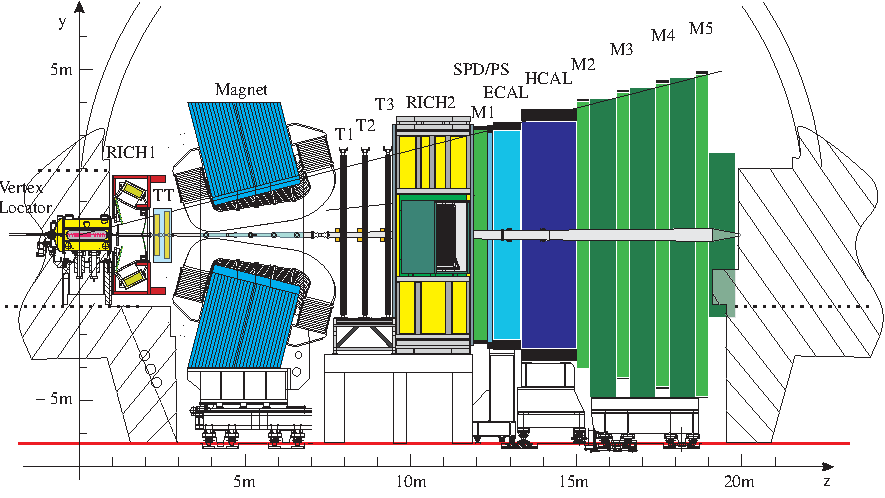
\includegraphics[width=0.95\textwidth]{./figs-detector/lhcb_detector_view.pdf}
    \caption{The LHCb detector.}
    \label{fig:lhcb-detector}
\end{figure}

still it is very efficient in capturing 40\% of \bbbar
this can be seen in the simuation FIGURE.

the detector has a high-precision tracking system with shit calorimeters and
other pid systems.
capable of resoution
